\documentclass[letterpaper]{article} % DO NOT CHANGE THIS
\usepackage[submission]{aaai2027} % DO NOT CHANGE THIS
\usepackage[hyphens]{url} % DO NOT CHANGE THIS
\usepackage{graphicx} % DO NOT CHANGE THIS
\urlstyle{rm} % DO NOT CHANGE THIS
\def\UrlFont{\rm} % DO NOT CHANGE THIS
\usepackage{natbib} % DO NOT CHANGE THIS AND DO NOT ADD ANY OPTIONS TO IT
\usepackage{caption} % DO NOT CHANGE THIS AND DO NOT ADD ANY OPTIONS TO IT
\usepackage{booktabs}
\usepackage{amsmath}
\usepackage{amssymb}
\frenchspacing % DO NOT CHANGE THIS

\pdfinfo{
/TemplateVersion (2027.1)
}

\setcounter{secnumdepth}{1}

\title{TerraState: A Testable Predictive-State World Model for Weather-Driven Land-Surface Forecasting}
\author{Anonymous Submission}
\affiliations{}

\begin{document}

\maketitle

\begin{abstract}
High-resolution satellite time series are a primary tool for monitoring vegetation, agriculture, and ecosystem response, and are increasingly cast as weather-driven forecasting: predicting future land-surface observations from cloud-obscured image histories and meteorological drivers. Yet such models are selected almost entirely by fixed-horizon pixel accuracy, which cannot establish whether their internal representations act as reusable world states rather than one-shot predictors. An accurate forecaster may still ignore the weather forcing, collapse toward persistence, or reach mutually incompatible states when the same interval is traversed directly versus in steps---failures that standard error metrics cannot detect. We introduce \textbf{TerraState}, a testable predictive-state world model that augments a forecasting backbone with a spatial state inferred from cloud-masked histories and a shared transition conditioned on future weather, geography, and elapsed time, requiring this state to carry the forecast. Rather than asserting a world state by architecture, TerraState makes it falsifiable through matched direct-versus-recursive forecasts, shuffled- and zeroed-driver controls, and direct-versus-composed consistency, each guarded by endpoint accuracy. On GreenEarthNet under temporal distribution shift, we report forecast skill---against persistence, video-prediction, and vegetation-forecasting baselines and a matched-backbone, matched-budget ablation---separately from these state diagnostics, turning the claim that a forecaster has learned a world state into a falsifiable question: whether an accurate forecaster also exposes a non-degenerate, driver-sensitive, and composition-consistent predictive state.
\end{abstract}

\section{Introduction}

High-resolution Earth-observation (EO) time series make localized vegetation dynamics directly observable, but only intermittently: optical acquisitions are sparse and often obscured by clouds, while the relevant land-surface response depends on weather and static geography. EarthNet2021 formalized this setting as guided video prediction from past Sentinel-2 observations, topography, and future meteorology \cite{requenamesa2021earthnet}. GreenEarthNet subsequently introduced a vegetation-focused cloud mask, a temporal-distribution-shift evaluation, and Contextformer, which combines a spatial vision backbone with weather-conditioned temporal prediction at 20\,m resolution \cite{benson2024multimodal}. Recurrent, convolutional, transformer, and diffusion models now provide strong alternatives for spatiotemporal forecasting \cite{shi2015convlstm,wang2017predrnn,gao2022simvp,gao2022earthformer,voleti2022mcvd}. Recent EO-specific work further models predictive uncertainty \cite{zhao2024vegediff}, structures meteorological forcing and evaluates response fidelity \cite{luo2026eowm}, or rolls a latent vegetation state under user-specified weather scenarios \cite{iele2026vegsim}.

\begin{figure*}[t!]
\centering
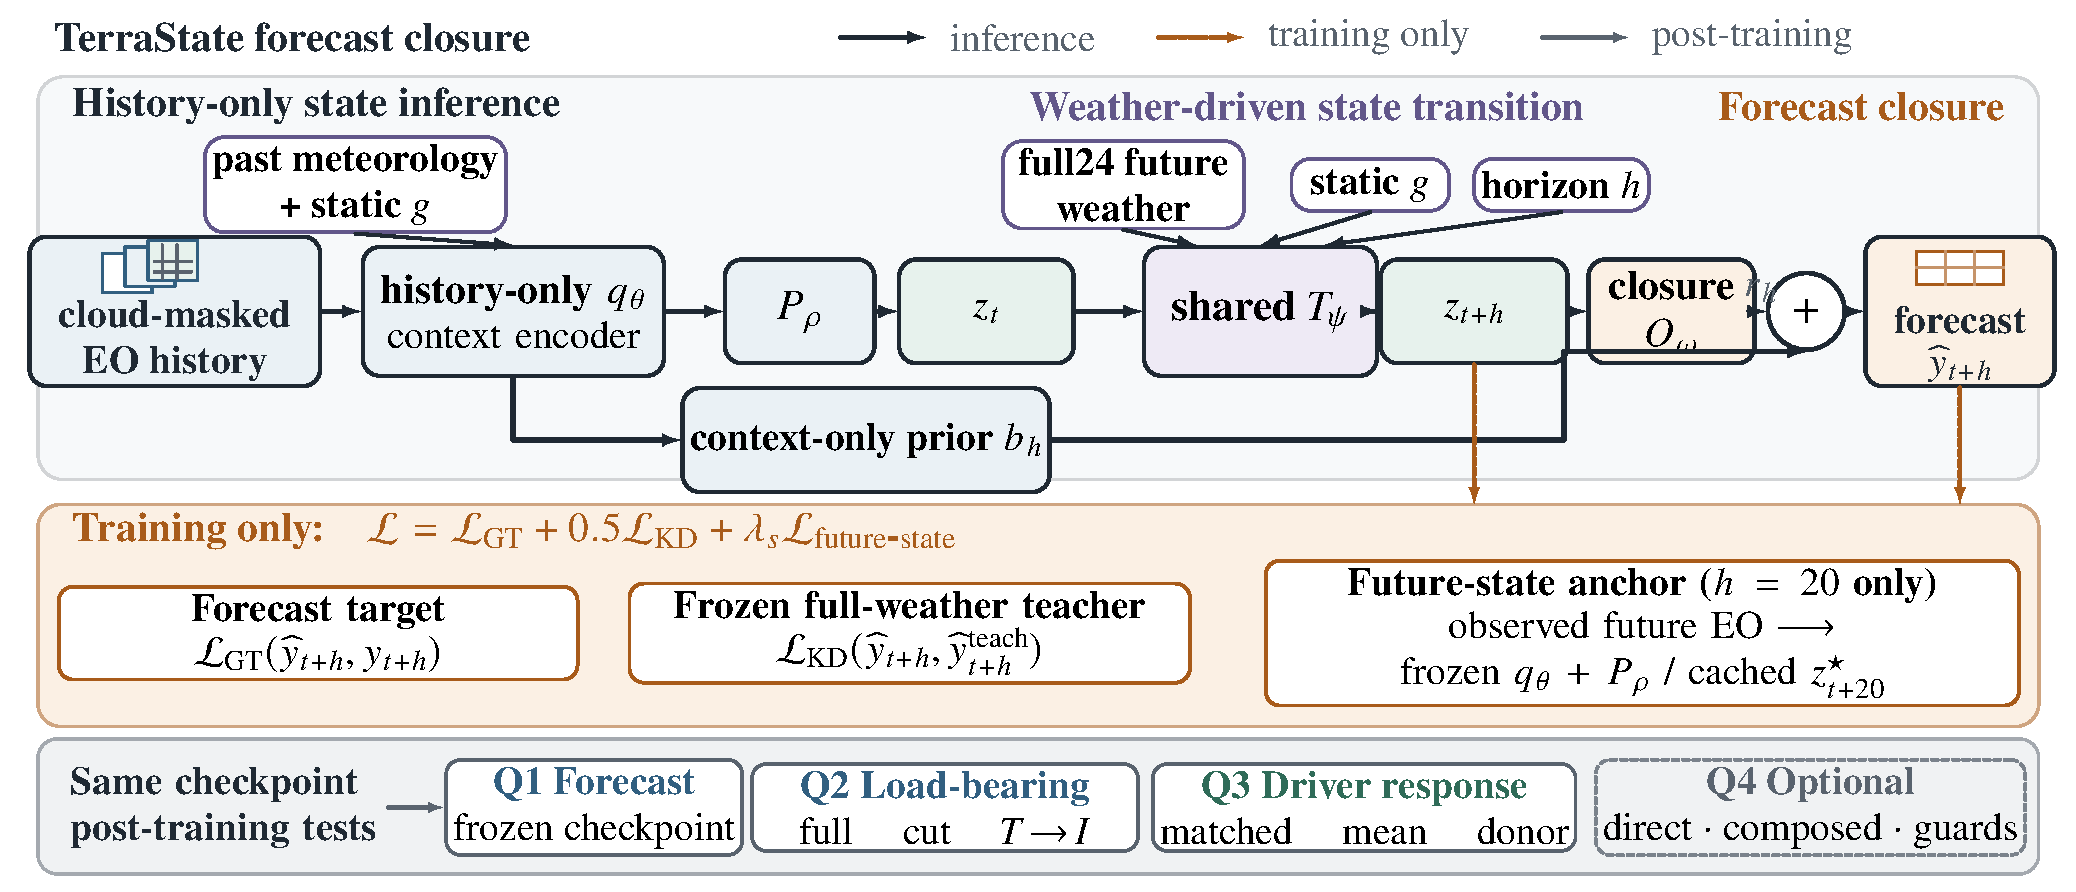
\includegraphics[width=0.98\textwidth]{../terrastate_overview_v3.pdf}
\caption{TerraState's solid inference path is history-only:
cloud-masked EO history, retained past meteorology, and static geography enter
$q_\theta$, which emits the context-only prior $b_h$ and, through $P_\rho$, the
spatial state $z_t$. Full24 future weather, static geography, and horizon $h$
condition the shared $T_\psi$; the state contribution
$O_\omega(z_{t+h})$ is then added explicitly to $b_h$. The orange band contains
only training supervision: the ground-truth forecast loss, distillation from a
frozen full-weather teacher, and the $h=20$ future-state anchor from a frozen
future-observation encoder/cache. Neither teacher nor observed future enters
inference. The bottom strip summarizes same-checkpoint post-training evidence:
Q1 forecast skill, Q2 closure and transition cuts, Q3 matched weather controls,
and optional Q4 direct/composed queries under endpoint and non-collapse guards.}
\label{fig:contract}
\end{figure*}

These advances sharpen a question that fixed-horizon forecast error does not answer: \emph{when does an accurate forecaster expose a state that can actually be advanced and reused?} A low pixel error can coexist with a representation that mainly copies the last clear observation, reacts weakly to future weather, or follows incompatible trajectories when the same forcing interval is traversed in one step or in several steps. General time-series evidence similarly shows that accurate forecasts can be supported by temporally disordered latent representations \cite{yang2026latenttsf}. In such cases, calling an internal feature a ``world state'' describes an architecture, not an empirically supported capability.

We argue that a predictive-state claim should be operational and falsifiable.
At minimum, the claimed state must contribute measurably to an accurate
endpoint forecast, and its shared transition must respond to the declared
exogenous driver. A stricter, optional test asks whether different partitions
of the same driver path reach compatible, accurate endpoints without identity
dynamics or representation collapse. These requirements are narrower than
claiming a complete physical state or a causal simulator. They are also
complementary to the output-level weather-response tests of
\citet{luo2026eowm} and the scenario-conditioned latent rollout of
\citet{iele2026vegsim}: those works ask whether outputs respond plausibly to
forcing, whereas we ask whether an exposed spatial state is load-bearing and
whether its shared transition withstands matched internal and endpoint tests.

TerraState implements this view with three components. A context operator
combines cloud-masked EO history, retained past meteorology, and static
geography to infer a spatial state; a single transition advances that state
under the 24-channel future-weather path, the same static geography, and
forecast horizon; and a forecast closure makes the transitioned state carry an
identifiable contribution beyond a context-only prior. Training aligns the
terminal transitioned state to a frozen representation of the observed future.
We separate ordinary forecasting skill (Q1) from load-bearing cuts (Q2) and
matched driver controls (Q3); direct-versus-composed path consistency and
anti-collapse measurements form an optional post-training extension (Q4).

Our contributions are:
\begin{itemize}
    \item We operationalize a predictive-state world model for weather-driven,
    high-resolution land-surface forecasting: a context-derived spatial state
    is advanced by one full24-conditioned shared transition and contributes to
    the endpoint forecast beyond a context-only prior.
    \item We anchor the transitioned state to a representation of the observed
    future produced by a frozen target encoder, connecting future-observation
    supervision to a state that remains on the forecast path at inference.
    \item We report forecast skill and state evidence separately for one selected
    checkpoint. Q1--Q3 test forecast sufficiency, load-bearing state use, and
    weather response; optional Q4 probes direct/composed reuse under endpoint
    and non-collapse guards. This is a matched verification protocol, not a new
    benchmark.
\end{itemize}

\section{Related Work}

\paragraph{Weather-driven EO forecasting.}
EarthNet2021 defines land-surface forecasting as future satellite prediction guided by meteorology \cite{requenamesa2021earthnet}; early analysis showed that explicit weather conditioning affects both forecast skill and simulated response \cite{diaconu2022weather}. GreenEarthNet and Contextformer focus the task on vegetation dynamics and introduce a strong multimodal, high-resolution baseline \cite{benson2024multimodal}. ConvLSTM, PredRNN, SimVP, and Earthformer represent recurrent-memory, convolutional, and transformer approaches commonly adapted to this task \cite{shi2015convlstm,wang2017predrnn,gao2022simvp,gao2022earthformer}. MCVD and VegeDiff instead model multiple plausible futures \cite{voleti2022mcvd,zhao2024vegediff}. ViT-Koop advances compressed EO states with a linear Koopman operator for efficient forecasting \cite{shinohara2025vitkoop}. TerraState instead places an exposed state in the forecast closure and tests, within the same checkpoint, whether that state is load-bearing and responds to the declared driver.

\paragraph{EO world models and forcing response.}
EO-WM frames EO forecasting as partially observed, weather-driven world modeling, decomposes climatology, anomalies, and accumulated stress, and evaluates extreme-summer and same-location cross-year response \cite{luo2026eowm}. VegSim is the closest architectural precedent: it infers a latent vegetation state, rolls it recurrently under future weather, and decodes NDVI quantiles for forecasting and scenario simulation \cite{iele2026vegsim}. Cloud-aware observability forecasting uses a latent world model for a different target---whether and when the next usable acquisition will occur \cite{albughdadi2026observability}. Complementing output-level response tests, TerraState ties an exposed state to the forecast itself, cuts that contribution under a matched checkpoint, and changes the forcing while tracking both state and output.

\paragraph{Predictive states and latent dynamics.}
Predictive-state representations define state through predictions of future observables rather than an unobserved physical variable \cite{littman2001predictive}. Modern world models learn compact dynamics for prediction and control \cite{ha2018worldmodels,hafner2019planet,hafner2020dreamer}, while joint-embedding architectures predict representations rather than raw pixels \cite{assran2023ijepa,bardes2024vjepa}. LatentTSF emphasizes state-space forecasting \cite{yang2026latenttsf}, and PLSM regularizes how controls change latent states \cite{saanum2024simplifying}. Deep-OSG studies semigroup-aware variable-time operators for autonomous systems \cite{chen2023deeposg}; concurrent work tests identity, inverse, and composition relations induced by group-structured agent actions \cite{wang2026groupactions}. Those algebraic settings differ from ordered, generally irreversible weather forcing; our optional path test therefore compares two partitions of the same observed forcing interval.

\paragraph{EO representation learning.}
Large-scale EO pretraining exploits seasons, multispectral time series, and cross-sensor views \cite{manas2021seco,cong2022satmae,wang2023ssl4eo,fuller2023croma,guo2024skysense}; cloud-removal work separately models uncertainty in optical time series \cite{ebel2023uncrtaints}. Such encoders can initialize the context operator, but a strong static representation does not by itself establish a forecast-bearing transition. Our diagnostics apply after the representation is placed on the forecasting path.

\section{Method}

\subsection{Problem Setting and Predictive-State Criterion}

Each example contains a cloud-obscured optical history
$\mathcal H_t=\{(x_i,m_i,\tau_i)\}_{i=1}^{C}$, a future meteorological path
$u_{t:t+H}$, static geographic context $g$, and future land-surface targets
$y_{t+1:t+H}$. Here $m_i$ marks valid pixels and $\tau_i$ records acquisition
time; $u_{a:b}$ uses half-open indexing and contains steps $a,\ldots,b-1$.
The public task uses $C=10$ five-day context observations and $H=20$
forecast endpoints \cite{benson2024multimodal}. Let
$\widetilde{\mathcal C}_t=(\mathcal H_t,u_{\leq t}^{\rm past},g)$ denote the
retained context: cloud-masked EO history, past meteorology, and static
geography, with future satellite frames, future target masks, and future
weather suppressed. TerraState represents a query at horizon $h$ as
\begin{equation}
\begin{aligned}
(b_{1:H},z_t)&=q_{\theta,\rho}(\widetilde{\mathcal C}_t),\\
z_{t+h}&=T_\psi(z_t,u_{t:t+h},g,h),\\
r_h&=O_\omega(z_{t+h}),\qquad
\widehat y_{t+h}=b_h+r_h ,
\end{aligned}
\label{eq:contract}
\end{equation}
where $b_h$ is a context-only forecast prior and $r_h$ is the contribution
carried by the transitioned state. Future weather can reach the final forecast
only through $T_\psi$; $b_h$ cannot change under a Q3 weather intervention.
Here $q_{\theta,\rho}$ denotes the composite context/state operator: below,
$q_\theta$ is its initialized forecasting backbone and $P_\rho$ its state
projector.

We call $z_t$ a \emph{predictive state} when it is inferred without future
target observations, contributes to endpoint prediction, and supports queries
under different horizons and forcing paths. The first two properties are
tested by the forecast and closure interventions; the third is probed by
matched weather changes and, optionally, path composition.

\subsection{Context-Only Spatial State}

To expose a spatial state without adding a second forecasting path, the
inference operator is initialized from a PVT v2/Contextformer forecaster
\cite{wang2022pvtv2,benson2024multimodal}. On
$\widetilde{\mathcal C}_t$ it embeds retained past meteorology and static
channels together with the cloud-masked EO context, returns a horizon-indexed
prior, and exposes the final context tokens before the forecast head. A spatial
projector converts those tokens into
\begin{equation}
z_t=P_\rho\!\left(
q_\theta(\widetilde{\mathcal C}_t)_{\mathrm{context\ end}}\right),
\qquad z_t\in\mathbb R^{N\times d}.
\label{eq:state}
\end{equation}
$P_\rho$ is a LayerNorm--linear--GELU--linear--LayerNorm projector with widths
$256\!\rightarrow\!512\!\rightarrow\!256$. $N$ indexes spatial patches and
$d$ is the state width. For a $128\times128$ minicube and $4\times4$ patches,
$(N,d)=(32^2,256)=(1024,256)$; the implementation flattens a batch to
$[1024B,256]$. Cloud masks determine which historical observations are usable.
Both the prior $b_{1:H}$ and state $z_t$ are computed from the same context-only
pass. This shared origin lets Q2 remove the state contribution while preserving
the history-conditioned prior; no second inference backbone or training teacher
is needed at test time.

\subsection{Shared Weather-Driven Transition}

The transition should attribute driver response to one reusable operator rather
than to separate horizon-specific heads. For a half-open interval $[a,b)$, a
shared GRU summarizes the \emph{ordered}
meteorological segment. Its input contains eight standardized E-OBS variables,
each aggregated by five-day mean, minimum, and maximum, for 24 channels.
Missing values are mapped to zero in this standardized space. Static geography
uses the three standardized elevation products averaged to the state patch
grid and passed through a two-layer MLP; elapsed time uses a fixed sinusoidal
embedding. The same static fields are available to $q_\theta$ in the retained
context and are separately encoded here for the transition:
\begin{equation}
e_{a:b}=E_u(u_{a:b}),\qquad
c_{a:b}=F\!\left(e_{a:b},E_g(g),E_h(b-a)\right).
\label{eq:condition}
\end{equation}
The three codes are fused by a two-layer MLP. One controlled residual
transition---LayerNorm followed by a three-layer GELU MLP with a residual
connection---is reused at every horizon and on every path:
\begin{equation}
T_\psi(z_a,u_{a:b},g,b-a)
=z_a+\Delta_\psi\!\left(\operatorname{LN}(z_a),c_{a:b}\right).
\label{eq:transition}
\end{equation}
Sharing $\psi$ across horizons makes its weather response testable in Q3.
Interval encoding preserves weather order and is recomputed for each
subinterval, which also permits the optional direct/composed query in Q4.

\subsection{Forecast Closure and Recoverability}

The closure places the transitioned state on the prediction path while retaining
an exact same-checkpoint removal test. It decodes each advanced spatial token
and unpatchifies the result into an endpoint residual:
\begin{equation}
r_h=O_\omega(z_{t+h}),\qquad
\widehat y_{t+h}^{(s)}=b_h+s\,r_h,\qquad s\in\{0,1\}.
\label{eq:closure}
\end{equation}
Normal inference fixes $s=1$; $s$ is not a learned gate. The diagnostic setting
$s=0$ exactly recovers the context-only prior while leaving the checkpoint and
sample population unchanged. TerraState therefore claims only that the state
carries a measurable forecast increment beyond $b_h$, not that every accurate
component of the forecast passes through $z_{t+h}$. The internal context-only
prior is also distinct from the separately trained matched-backbone comparator
used in Q1.

\subsection{Optional Direct and Composed Evaluation Queries}

To test whether the shared transition can be reused over subintervals, for
$h=h_1+h_2$ TerraState exposes two paths from the same state under the same
ordered forcing:
\begin{align}
z_h^{\mathrm{dir}}
&=T_\psi(z_t,u_{t:t+h},g,h), \label{eq:direct}\\
z_h^{\mathrm{cmp}}
&=T_\psi\!\left(
T_\psi(z_t,u_{t:t+h_1},g,h_1),
u_{t+h_1:t+h},g,h_2\right).
\label{eq:composed}
\end{align}
The direct path applies $T_\psi$ once over the full interval; the composed path
reuses it over an evaluation partition. Both states are closed to forecasts
$\widehat y_h^{\mathrm{dir}}$ and $\widehat y_h^{\mathrm{cmp}}$ and compared
with the same true endpoint $y_h$. These queries are never optimized: after
training and checkpoint selection, optional Q4 applies them to a predeclared
evaluation set $\mathcal P_{\mathrm{Q4}}$. Agreement therefore measures
post-training behavior rather than a composition objective seen during
optimization.

\subsection{Training Objective and Curriculum}

Training proceeds in three phases after \emph{forecast initialization}
warm-starts the PVT/Contextformer context operator and compatible TerraState
modules from a forecasting checkpoint. We train for 40 epochs and 14,880
optimizer updates
(372 updates per epoch). In phase 1, steps $[0,2976)$, $q_\theta$ is frozen and
$\lambda_s$ rises linearly from 0 to 0.02. In phase 2, steps
$[2976,11904)$, $q_\theta$ remains frozen and $\lambda_s=0.02$; a checkpoint is
forced at the 80\% boundary. In phase 3, steps $[11904,14880)$, only
\texttt{core.blocks.2}, the final Transformer block of $q_\theta$, is
unfrozen and $\lambda_s=0.01$. All earlier blocks remain frozen.

Optimization uses AdamW with $\beta=(0.9,0.999)$, zero weight decay, and
global batch 64 (eight GPUs, eight samples per GPU, no gradient accumulation).
The non-$q$ branch has base learning rate $3\times10^{-5}$; the $q$ parameter
group uses $0.033$ times that rate, $9.9\times10^{-7}$, and receives updates
only in phase 3. A shared multiplier warms linearly from zero for 300 optimizer
steps and then follows cosine decay; gradients are clipped at norm 1.0.
Validation-only selection freezes one checkpoint for Q1--Q3, optional Q4, and
the one-shot temporal-shift evaluation.

Let $\mathcal P$ be the vegetation pixels with a valid prediction and
$v_{p,h}\in\{0,1\}$ indicate that pixel $p$ is clear at horizon $h$. The
forecast loss first averages over the visible horizons of each pixel and then
averages over pixels:
\begin{equation}
\mathcal L_{\mathrm{GT}}
=\frac{1}{|\mathcal P|}\sum_{p\in\mathcal P}
\frac{\sum_{h=1}^{H}v_{p,h}(\widehat y_{p,h}-y_{p,h})^2}
{\sum_{h=1}^{H}v_{p,h}+\epsilon}.
\label{eq:gtloss}
\end{equation}
A strong full24 forecasting teacher is frozen throughout training and
discarded at inference. Its prediction
$\widehat y_h^{\,\mathrm{teach}}$ supplies the single knowledge-distillation
term
\begin{equation}
\mathcal L_{\mathrm{KD}}
=\frac{\sum_{p,h}v_{p,h}
(\widehat y_{p,h}-\operatorname{sg}(\widehat y_{p,h}^{\,\mathrm{teach}}))^2}
{\sum_{p,h}v_{p,h}+\epsilon}.
\label{eq:kdloss}
\end{equation}
Future-state supervision is generated before optimization by a frozen copy of
the initialized $q_\theta$ and $P_\rho$. For valid terminal patches
$i\in\{1,\ldots,1024B\}$ with mask $m_i$, it is
\begin{equation}
\begin{aligned}
z^*_{t+20,i}
&=\operatorname{sg}\!\left[
P_{\mathrm{frozen}}\!\left(
q_{\mathrm{frozen}}(o_{\leq t+20})\right)_i\right],\\
\ell_i^{\mathrm{state}}
&=1-\cos\!\left(
\operatorname{LN}(z_{t+20,i}),
\operatorname{LN}(z^*_{t+20,i})\right),\\
\mathcal L_{\mathrm{future\text{-}state}}
&=\frac{\sum_i m_i\ell_i^{\mathrm{state}}}
{\sum_i m_i+\epsilon}.
\end{aligned}
\label{eq:futurestate}
\end{equation}
The target input contains the observed future EO sequence, has future weather
zeroed, and supplies only the terminal $h=20$ target. A terminal $4\times4$
patch is valid only if it is fully cloud-free and contains at least one
vegetation pixel. Each cube's $[1024,256]$ target is cached in FP16 together
with its Boolean mask, relative source path, and provenance checksums. Targets
are computed once into separate train and validation caches, and training
consumes only those cached tensors. Neither the target encoder nor the
forecasting teacher is part of the inference model. The only nonzero training
objective is
\begin{equation}
\begin{aligned}
\mathcal L
&=\mathcal L_{\mathrm{GT}}
+0.5\,\mathcal L_{\mathrm{KD}}
+\lambda_s\,\mathcal L_{\mathrm{future\text{-}state}},\\
\lambda_s&=
\begin{cases}
\text{linear }0\rightarrow0.02, & 0\% \text{--}20\%,\\
0.02, & 20\% \text{--}80\%,\\
0.01, & 80\% \text{--}100\%.
\end{cases}
\end{aligned}
\label{eq:total}
\end{equation}
Q2--Q4 cuts, weather interventions, path comparisons, and non-collapse
statistics are post-training measurements and receive no gradient. In
particular, future-state supervision is a training signal rather than evidence
that Q2 has passed; load-bearing state use must still be established by
endpoint interventions.

\subsection{Matched State Diagnostics}

\paragraph{Load-bearing.}
We report full, closure-cut, and transition-to-identity forecasts on identical
samples. The closure cut sets the state-carried increment to zero
($s=0$ in Equation~\ref{eq:closure}) and therefore recovers $b_h$ without
altering the inferred state. The transition cut replaces $T_\psi$ by the
identity while keeping the closure, decoder, and all other inputs fixed. A state
is credited as load-bearing only if these cuts remove a measurable paired
full-versus-reference gain and change the endpoint output. Because
$T\!\rightarrow I$ can feed $O_\omega$ a state outside its trained input
distribution, the exact closure cut is primary and the transition cut is
supporting mechanism evidence.

\paragraph{Driver sensitivity.}
Matched future weather is compared with (i) a season- and geography-matched,
distinct donor sequence and (ii) the normalized-mean control obtained by
zeroing weather after the fixed centering transform. The donor manifest,
matching keys, and normalization record are set from validation before test evaluation. We
keep history, geography, reference forecast, masks, and checkpoint fixed;
change only the declared transition input; and report paired changes in
transitioned state, endpoint output, and forecast score. An unmatched
within-batch shuffle is used only for engineering smoke tests.

\paragraph{Optional post-training path consistency with endpoint guards.}
After freezing the checkpoint, for each predeclared Q4 partition $p$ we report
direct and composed endpoint errors
$E_p^{\mathrm{dir}}$ and $E_p^{\mathrm{cmp}}$ separately. The metric and
thresholds are fixed on validation data. A partition qualifies only when both
endpoints satisfy the absolute guard and the composed path meets a
predeclared non-inferiority margin:
\begin{equation}
G_p=\mathbb 1\!\left[
\begin{aligned}
&\max(E_p^{\mathrm{dir}},E_p^{\mathrm{cmp}})
\leq\tau_{\mathrm{abs}}\\[-1mm]
&{}\wedge\
E_p^{\mathrm{cmp}}\leq(1+\epsilon_{\mathrm{NI}})E_p^{\mathrm{dir}}
\end{aligned}
\right].
\label{eq:endpointguard}
\end{equation}
For qualified partitions, we report
\begin{equation}
\begin{aligned}
\delta_z&=\operatorname{mean}|z_h^{\mathrm{dir}}-z_h^{\mathrm{cmp}}|,\\
\delta_y&=\ell_{\mathcal V_h}
(\widehat y_h^{\mathrm{dir}},\widehat y_h^{\mathrm{cmp}}),\\
A_{\mathrm{comp}}&=\delta_y^{\mathrm{broken}}-\delta_y .
\end{aligned}
\label{eq:pathmetric}
\end{equation}
The real second leg consumes $u_{t+h_1:t+h_1+h_2}$. The broken control instead
feeds that leg the equal-length prefix $u_{t:t+h_2}$, while retaining its
elapsed-time embedding $h_2$; the first leg, direct path, geography, prior,
closure, and target are unchanged. The half-open windows neither duplicate nor
drop a boundary step on the real path. Thus
$A_{\mathrm{comp}}$ asks whether the real path agrees better than a deliberately
misaligned path. Path agreement is withheld from positive interpretation
whenever $G_p=0$, and Q4 cannot compensate for a failed Q2.

\paragraph{Non-degeneracy.}
Within each minicube, we compute mean absolute movement
$M_h=\operatorname{mean}_{n,c}|z_{t+h,n,c}-z_{t,n,c}|$, average the
per-channel standard deviation across patch tokens to obtain $S_h$, and form
the patch-token covariance after channel-wise centering. Its effective rank is
\begin{equation}
r_{\mathrm{eff}}=
\frac{(\sum_i\lambda_i)^2}{\sum_i\lambda_i^2+\epsilon},
\label{eq:erank}
\end{equation}
where $\lambda_i$ are eigenvalues of the patch-token covariance. We also report
$S_h/S_t$ and $r_{\mathrm{eff},h}/r_{\mathrm{eff},t}$. These quantities guard
against identity dynamics, constant states, and deceptively low path gaps. They
are computed at horizons $\{1,5,10,20\}$ on the same minicubes used by the path
test and then averaged over minicubes; across-minicube movement variance is
retained as an additional audit field.

\section{Experiments}

\subsection{Questions and Protocol}

Following the claim structure, the experiments answer four predeclared
questions:
\begin{enumerate}
    \item \textbf{Q1---Forecast skill:} Is the selected TerraState checkpoint competitive under temporal distribution shift and against the matched backbone?
    \item \textbf{Q2---Load-bearing:} Does cutting the state-carried contribution or its transition remove a measurable forecasting contribution?
    \item \textbf{Q3---Driver sensitivity:} Does matched weather improve prediction relative to matched-donor and normalized-mean forcing?
    \item \textbf{Q4---Optional composition and non-collapse:} After training,
    are direct/composed queries individually accurate, mutually compatible, and
    non-degenerate?
\end{enumerate}

\paragraph{Data and validation-only selection.}
We use GreenEarthNet \cite{benson2024multimodal}. Each minicube contains
$30$ five-day Sentinel-2 composites at $128\times128$ pixels and 20\,m ground
sampling, aligned meteorology, a cloud/quality mask, and elevation. The first
$10$ composites form the context and the following $20$ define the target
horizon. Architecture, loss, decision thresholds, the donor rule, and
checkpoint selection use training and validation data only. The donor rule
specifies its season, geography, day-of-year window, reuse cap, and
divergence-quantile level before temporal-shift evaluation. The per-track
assignment and its absolute divergence floor are then computed
deterministically from input-side time, location, and provided future weather
before model scoring; they never use targets, predictions, or errors. This
transductive use of declared test covariates is recorded and hashed. After the
remaining choices are fixed, the selected checkpoint is evaluated once on the
available \texttt{ood-t\_chopped} temporal-shift track with 1,904 minicubes;
this track is never used for checkpoint selection, early stopping, or
performance-threshold tuning. We do not describe this subset as the complete
GreenEarthNet protocol because the local evaluation bundle does not contain
every official split.

\paragraph{Targets and metrics.}
The primary target is NDVI over pixels that are both valid and in the declared
vegetation land-cover range. We report $R^2$, RMSE, NSE, absolute bias,
outperformance, and RMSE25 using one fixed scorer and one aggregation
convention. NSE is Nash--Sutcliffe efficiency; RMSE25 is RMSE over the first
five five-day endpoints; and outperformance is the fraction of aligned
minicube--land-cover groups that beat the fixed climatology reference on at
least three of four prescribed criteria. EarthNetScore, when used for an
optional EarthNet2021 analysis, is reported in a separate table and never
mixed with GreenEarthNet metrics.

\paragraph{Comparisons.}
Published baselines are transcribed from the GreenEarthNet/Contextformer report
\cite{benson2024multimodal} and labeled Reported. They provide historical
context only. The exact local panel contains the already available matched
forecasting backbone and the selected TerraState checkpoint; no local reproduction
of ConvLSTM, PredRNN, SimVP, Earthformer, or Contextformer is required. Every
paired claim is restricted to these local rows sharing target files, masks,
horizons, scorer, and aggregation code. The matched backbone uses the same forecasting
lineage and declared local protocol but omits TerraState's state projector,
transition, and closure; any remaining budget or teacher-access difference is
reported as a confound. We never claim a strict ranking across the published
and local panels.

\paragraph{Implementation and statistics.}
TerraState uses a context-only PVT/Contextformer prior, a projected
spatial state, the shared transition in Equation~\ref{eq:transition}, and the
residual closure in Equation~\ref{eq:closure}. It contains 7,180,896 unique
\texttt{nn.Parameter} scalars, including the frozen $q$ backbone but excluding
buffers (including the fixed closure coefficient), the frozen KD teacher, the
offline future-target encoder, and its cache. Of these, 1,120,336 are trainable
in phases 1--2 and 1,910,096 in phase 3. Its per-minicube state shape is
$[1024,256]$ (runtime $[1024B,256]$). The 40-epoch, 14,880-update AdamW
configuration, learning-rate groups, batch 64, and three-phase schedule are
specified above; the checkpoint is selected on \textbf{[FROZEN FULL-VALIDATION
CRITERION]}. The primary Q1--Q3 report and optional Q4 use this one checkpoint
and paired minicube-level bootstrap intervals. If
\textbf{[REPLICATION SEEDS]} independent replications are completed, they are
secondary robustness evidence, not an average substituted for the
checkpoint-level state claim; without them, Q1 is labeled a single-checkpoint
comparison rather than a general training-stability claim. Before the one-shot
test, the reproducibility record stores hashes for the student initialization,
training-only teacher, frozen future-target encoder/projector and target-cache
manifest, final checkpoint, serialized model configuration, three-term
objective configuration, validation selection record, data manifest,
evaluator, mask/aggregation protocol, donor manifest, endpoint guard, and
optional Q4 evaluation partitions.

\begin{table*}[t]
\centering
\small
\setlength{\tabcolsep}{2.0pt}
\begin{tabular}{llcccccc}
\toprule
Method & Source & $R^2\uparrow$ & RMSE$\downarrow$ & NSE$\uparrow$ &
$|\mathrm{Bias}|\downarrow$ & RMSE25$\downarrow$ & Outperf.$\uparrow$\\
\midrule
\multicolumn{8}{l}{\emph{A. Published context (reported values)}}\\
Persistence & Reported & 0.00 & 0.23 & $-1.28$ & 0.17 & 0.09 & 21.8\%\\
Previous year & Reported & 0.56 & 0.20 & $-0.40$ & 0.14 & 0.18 & 19.3\%\\
Climatology & Reported & 0.58 & 0.18 & $-0.34$ & 0.13 & 0.16 & n.a.\\
ConvLSTM & Reported & $0.58{\pm}0.01$ & $0.16{\pm}0.00$ &
$-0.13{\pm}0.02$ & $0.11{\pm}0.00$ & $0.11{\pm}0.00$ &
$53.1{\pm}1.2$\%\\
Earthformer & Reported & 0.52 & 0.16 & $-0.13$ & 0.10 & 0.09 & 56.5\%\\
PredRNN & Reported & $0.62{\pm}0.00$ & $0.15{\pm}0.00$ &
$0.03{\pm}0.00$ & $0.10{\pm}0.00$ & $0.10{\pm}0.00$ &
$64.7{\pm}1.2$\%\\
SimVP & Reported & $0.60{\pm}0.00$ & $0.15{\pm}0.00$ &
$0.03{\pm}0.01$ & $0.09{\pm}0.00$ & $0.10{\pm}0.00$ &
$64.1{\pm}1.0$\%\\
Contextformer & Reported & $0.62{\pm}0.00$ & $0.14{\pm}0.00$ &
$0.09{\pm}0.01$ & $0.09{\pm}0.00$ & $0.08{\pm}0.00$ &
$66.8{\pm}0.3$\%\\
\midrule
\multicolumn{8}{l}{\emph{B. Exact local protocol (paired comparison only)}}\\
Matched backbone & Local & TBD & TBD & TBD & TBD & TBD & TBD\\
\textbf{TerraState} & Local & TBD & TBD & TBD & TBD & TBD & TBD\\
\bottomrule
\end{tabular}
\caption{Published forecast context and the local temporal-shift comparison.
Panel A transcribes reported values from Table 2 of
\citet{benson2024multimodal}; reported standard deviations use three seeds
where available. Panel B contains only the matched backbone and TerraState under one
local manifest and evaluator. Different protocols preclude strict cross-panel
ranking. TerraState's Q1--Q3 and optional Q4 results refer to the same frozen
checkpoint; local confidence intervals and paired win/tie/loss counts accompany
the machine-readable package.}
\label{tab:forecast}
\end{table*}

\subsection{Q1: Forecast Skill under Temporal Shift}

Table~\ref{tab:forecast} separates published context from the exact local
matched comparison. The
final result paragraph will make only one of three evidence-supported claims:
(i) improvement over the matched backbone with a paired confidence interval,
(ii) validation-predeclared non-inferiority together with an additional state
capability, or (iii) a negative result that triggers claim reduction. Without a
predeclared margin, option (ii) is unavailable. The paragraph will not mix the
published Contextformer aggregation with a locally computed score or describe
a single-seed pilot as state of the art.

% RESULT TEMPLATE Q1--PASS: report exact-protocol gain and paired interval.
% RESULT TEMPLATE Q1--PARTIAL: report a predeclared non-inferiority result, or
% descriptive parity if no margin was frozen; do not call the latter non-inferior.
% RESULT TEMPLATE Q1--FAIL: report the deficit and downgrade the practical claim.
% RESULT FILL: On [N] test minicubes, the frozen TerraState checkpoint obtains
% [METRICS]. Relative to the matched backbone, the paired minicube difference is
% [DELTA, CI], with [W/T/L] wins/ties/losses. The identical checkpoint is used
% in all diagnostics below.

\subsection{Q2--Q3: Load-Bearing State and Weather Response}

Table~\ref{tab:cuts} separates absolute forecast accuracy from the incremental
contribution of the state branch. Q2 compares the full checkpoint with its
recoverable closure cut and a transition-to-identity cut; the matched backbone
remains the Q1 reference. Q3 changes only the declared transition input while
holding history, geography, closure, masks, sample population, and checkpoint
fixed.

\begin{table*}[t]
\centering
\small
\setlength{\tabcolsep}{4pt}
\begin{tabular}{llcccccc}
\toprule
Test & Variant & $R^2\uparrow$ & RMSE$\downarrow$ &
$\Delta_{\rm loss}R^2$ & $\Delta_{\rm rise}$RMSE &
State $|\Delta|$ & Output $|\Delta|$\\
\midrule
Q2 & Full TerraState & TBD & TBD & 0 & 0 & 0 & 0\\
Q2 & Closure cut & TBD & TBD & TBD & TBD & -- & TBD\\
Q2 & $T\!\rightarrow\!I$ cut & TBD & TBD & TBD & TBD & TBD & TBD\\
\midrule
Q3 & Matched weather & TBD & TBD & 0 & 0 & 0 & 0\\
Q3 & Normalized-mean weather & TBD & TBD & TBD & TBD & TBD & TBD\\
Q3 & Season/geography donor & TBD & TBD & TBD & TBD & TBD & TBD\\
\bottomrule
\end{tabular}
\caption{Matched Q2--Q3 interventions on identical samples. Q2 deltas are
full-minus-variant for $R^2$ and variant-minus-full for RMSE; Q3 uses matched
weather as reference, so positive means lost skill. State/output columns are
mean absolute token/valid-pixel NDVI changes, and the Q3 context prior must be
invariant. Because the closure cut equals that prior, we report its absolute
paired effect rather than an algebraic ``gain removed fraction.'' Per-horizon
values and intervals accompany the table.}
\label{tab:cuts}
\end{table*}

% RESULT TEMPLATE Q2/Q3--PASS: both cuts have practical paired effects and
% matched weather beats both controls with state and output changes.
% RESULT TEMPLATE Q2/Q3--PARTIAL: name exactly which subclaim is supported and
% withhold the unsupported forecast-bearing or driver-sensitive adjective.
% RESULT TEMPLATE Q2/Q3--FAIL: report null/adverse effects and reject that subclaim.
% RESULT FILL: The closure cut changes [PRIMARY METRIC] by [ABSOLUTE DELTA, CI].
% The transition cut changes endpoint predictions by [VALUE, CI],
% [SUPPORTING/NOT SUPPORTING] a load-bearing state. Matched weather
% [OUTPERFORMS/DOES NOT OUTPERFORM] normalized-mean forcing by [DELTA, CI] and
% the season/geography-matched donor by [DELTA, CI]; corresponding state and
% output changes are [SUMMARY].

\subsection{Optional Post-Training Q4: Composition and Anti-Collapse}

Q4 is a post-training extension and may be moved to the supplementary
document. It uses the validation-frozen partition set
\[
\mathcal P_{\mathrm{Q4}}=\{(3,7),(6,4),(4,11),(8,12),(2,18)\}
\]
only after the
unique checkpoint has been selected and frozen; these partitions do not define
training examples or losses. Every partition is evaluated on the same endpoint
population. A row receives a positive path-consistency interpretation only if
its direct and composed endpoints pass Equation~\ref{eq:endpointguard}, its
real output gap is compared with the asymmetric broken-path control, and the
state-retention measurements do not indicate collapse. Q4 neither changes the
checkpoint nor participates in model selection.

\begin{table*}[!t]
\centering
\small
\setlength{\tabcolsep}{2.1pt}
\begin{tabular}{lccccccc}
\toprule
\multicolumn{8}{l}{\emph{A. Endpoint accuracy and path controls by partition}}\\
Partition & $E^{\rm dir}$ & $E^{\rm cmp}$ & Joint guard &
$\delta_z$ & $\delta_y$ & $\delta_y^{\rm broken}$ & $A_{\rm comp}$\\
\midrule
3+7 & TBD & TBD & TBD & TBD & TBD & TBD & TBD\\
6+4 & TBD & TBD & TBD & TBD & TBD & TBD & TBD\\
4+11 & TBD & TBD & TBD & TBD & TBD & TBD & TBD\\
8+12 & TBD & TBD & TBD & TBD & TBD & TBD & TBD\\
2+18 & TBD & TBD & TBD & TBD & TBD & TBD & TBD\\
\midrule
\multicolumn{8}{l}{\emph{B. Anti-collapse summaries by direct-query horizon}}\\
Horizon & $M_h$ & $S_h/S_t$ & $r_{\rm eff,h}/r_{\rm eff,t}$ &
\multicolumn{4}{c}{Validation-frozen degeneracy check}\\
\midrule
1 & TBD & TBD & TBD & \multicolumn{4}{c}{TBD}\\
5 & TBD & TBD & TBD & \multicolumn{4}{c}{TBD}\\
10 & TBD & TBD & TBD & \multicolumn{4}{c}{TBD}\\
20 & TBD & TBD & TBD & \multicolumn{4}{c}{TBD}\\
\bottomrule
\end{tabular}
\caption{Optional post-training Q4 separates partition-level path evidence
(A) from horizon-level anti-collapse evidence (B). No Q4 quantity is a
training loss or selection criterion. Panel A reports endpoint MSE, the joint
guard, state/output gaps, the broken-path gap, and
$A_{\mathrm{comp}}=\delta_y^{\mathrm{broken}}-\delta_y$. Panel B reports
movement, standard-deviation retention, effective-rank retention, and the
validation-frozen degeneracy check. Positive interpretation requires a passing
joint guard and cannot compensate for failed Q2.}
\label{tab:composition}
\end{table*}

% RESULT TEMPLATE Q4--PASS: all predeclared endpoint guards pass, the real path
% beats the broken control, and state retention excludes the declared degeneracies.
% RESULT TEMPLATE Q4--PARTIAL: name passing partitions and withhold general path reuse.
% RESULT TEMPLATE Q4--FAIL: report failed guards/control/retention and reject Q4 support.
% RESULT FILL: On predeclared Q4 partitions, [NUMBER] of [TOTAL] rows pass the
% endpoint and non-inferiority guards. The pooled A_comp is [VALUE, CI], with
% [NUMBER] row-wise real/broken ratios below one. Transition movement, state
% standard-deviation retention, and effective-rank retention [DO/DO NOT]
% exclude the declared identity or collapsed solutions.

\subsection{Same-Checkpoint Diagnostics and Optional External Analyses}

The required mechanism evidence uses the selected checkpoint without
retraining: Q2 applies the closure and $T\!\rightarrow I$ cuts, while Q3 changes
only the future-weather input. We do not require retrained removals of the
projector, transition, conditioning encoders, KD term, or future-state anchor
for the main claims. If later conducted, such studies will be labeled
supplementary rather than substituted for Q1--Q3. Independent EO-WM response
protocols \cite{luo2026eowm} are likewise optional external analyses, not part
of the required evidence.

\paragraph{Qualitative analysis.}
A qualitative panel is included only after real arrays are available. It uses
one validation-selected tile and shows target NDVI, full/closure-cut forecasts,
matched/donor change, and direct/composed change on shared scales with
valid-pixel coverage. The identifier is frozen before test scoring and is
never chosen from test errors or saliency.

\section{Limitations and Scope}

TerraState learns a future-predictive representation constrained by satellite
history and supplied meteorology; it does not recover a complete physical
land-surface state. Future weather in the benchmark is an oracle exogenous
input, so operational performance with forecast rather than observed weather
may be lower.

Matched-versus-donor sensitivity measures conditional response, not causal
identification or counterfactual correctness. Direct/composed agreement is an
empirical finite-horizon diagnostic, not a proof of physical validity,
associativity, or a semigroup law. The residual closure supports only the claim
that the state-mediated branch carries a measurable forecast increment, not
that every accurate output component or the history content of $z_t$ is
indispensable. Because Q4 is not optimized, failure of its optional
post-training test limits any composition claim but does not overwrite the
separately reported Q1--Q3 findings.

The contract is a matched verification protocol for the selected TerraState
checkpoint, not an independent benchmark, and one temporal-shift track cannot
establish cross-dataset generality. Optical targets also remain affected by
cloud screening and unobserved variables such as soil moisture, irrigation,
and vegetation type.

\section{Conclusion}

TerraState makes a world-state claim falsifiable: one accurate checkpoint must
expose a load-bearing state whose shared transition uses the declared weather
driver. Q1--Q3 test these core claims; optional Q4 probes guarded composition.

\bibliography{references}

\end{document}
